\documentclass[10pt]{beamer}
\usepackage{graphicx}
\usepackage{amsmath}
\usepackage{bm}
\usepackage{hyperref}
\usepackage{booktabs}
\usepackage{color}
\usepackage{xcolor}
\usepackage{amssymb}      % For \checkmark
\usepackage[utf8]{inputenc} % For ° and £ (or use \pounds)
\usepackage{tikz}
\usetikzlibrary{shapes.geometric, arrows, positioning, calc, fit, backgrounds}

% Enable speaker notes (uncomment one of these options)
%\setbeameroption{show notes} % Notes on separate pages
\setbeameroption{show notes on second screen=right} % Notes on second screen for presentation
\usepackage{pgfpages}

% TikZ styles for block diagrams
\tikzstyle{startstop} = [rectangle, rounded corners, minimum width=3cm, minimum height=1cm,text centered, draw=black, fill=red!30]
\tikzstyle{process} = [rectangle, minimum width=3cm, minimum height=1cm, text centered, text width=3cm, draw=black, fill=blue!20]
\tikzstyle{sensor} = [rectangle, minimum width=2.5cm, minimum height=0.8cm, text centered, text width=2.5cm, draw=black, fill=green!20]
\tikzstyle{power} = [rectangle, minimum width=2.5cm, minimum height=0.8cm, text centered, text width=2.5cm, draw=black, fill=yellow!30]
\tikzstyle{arrow} = [thick,->,>=stealth]

\usetheme{Boadilla}

\title{Free-Roving Subsea Cable Inspection Drone}
\subtitle{A Technical Feasibility Study}
\author{Jerry Liu (yhl63) \\ Zihe Liu (zl559)}
\institute{University of Cambridge}
\date{\today}

% Custom footnote settings
\setbeamercolor{footline}{use=structure,bg=structure.fg, fg=white}
\setbeamertemplate{footline}{%
  \leavevmode%
  \begin{beamercolorbox}[wd=\paperwidth,ht=2.5ex,dp=1ex]{footline}%
    \hfill
    \insertshorttitle
    \hfill
    \insertframenumber/\inserttotalframenumber
    \hspace{1em}
  \end{beamercolorbox}%
}

% Add section divider slides
\AtBeginSection{
  \begin{frame}
  \vfill
  \centering
  \begin{beamercolorbox}[sep=8pt,center,shadow=true,rounded=true]{title}
    \usebeamerfont{title}\insertsectionhead\par%
  \end{beamercolorbox}
  \vfill
  \end{frame}
}

\begin{document}

% Title slide
\frame{\titlepage}

%%%%%%%%%%%%%%%%%%%%%%%%%%%%%%%%%%%%%%%%%%%%%%%%%%%%%%%%%%%%%%%%%%%%%
\section{The Problem - Subsea Cable Inspection}

\begin{frame}{The Problem - Why Subsea Cables Matter}
  \begin{columns}[T]
    \begin{column}{0.45\textwidth}
      \textbf{Backbone of the Internet:}
      \begin{itemize}
        \item 97-99\% of intercontinental data traffic
        \item 500+ cables worldwide
        \item 14 million kilometers total
        \item 2-5 cm diameter (garden hose size)
      \end{itemize}
    \end{column}
    \begin{column}{0.52\textwidth}
      \includegraphics[width=\textwidth]{img/subsea_cables.png}
    \end{column}
  \end{columns}

  \note{Before we dive into our design and feasibility assessment, let's give some context to the problem we're tackling: Subsea cables. Your internet connection, whether that be for online banking or video calls, 97-99\% of that data goes through a dense network of over 500+ undersea cables, spanning a total of 14 million kilometers over the seafloor making it THE largest and possibly greatest man-made infrastructure ever. This is the backbone of the internet, and when they fail, the consequences are severe. Despite the significance of these cables, these cables are no thicker than your average garden-hose around 2-5 cm in diameter, with hair-thin strands of optical fiber embedded within, designed to remain undisturbed across the seabed.}
\end{frame}

\begin{frame}{The Problem - Current Limitations}
  \begin{columns}[T]
    \begin{column}{0.55\textwidth}
      \includegraphics[width=\textwidth]{img/ship.png}
    \end{column}
    \begin{column}{0.42\textwidth}
      \textbf{Cable Faults:}
      \begin{itemize}
        \item ~200 faults/year
        \item Shallow waters most vulnerable
        \item Shetland Islands 2022: 23,000 people offline
      \end{itemize}

      \vspace{0.5em}

      \textbf{Traditional: Tethered ROVs}
      \begin{itemize}
        \item[+] Unlimited power
        \item[+] Real-time comms
        \item[--] Limited range
        \item[--] Tether entanglement
        \item[--] High operational cost
      \end{itemize}
    \end{column}
  \end{columns}

  \vspace{0.5em}
  \centering
  \colorbox{yellow!30}{\textbf{Solution: Free-roving Autonomous Underwater Vehicle}}

  \note{In shallow waters however, these subsea cables are susceptible to a wider range of disturbances, largely from human activities such as anchoring, or snagged by nets, resulting in roughly 200 faults a year. In October 2022, both cables serving the Shetland Islands were damaged. For days, 23,000 people had no internet, could not use card payments, could not access online banking. Businesses lost thousands. Emergency services were disrupted. These are not rare events, they require constant monitoring and effective maintenance. When a fault occurs, an army of ships strategically placed around the world would identify and repair the location of the fault, which usually involves the usage of a tethered drone to inspect the damaged cable. Despite the effectiveness of tethered communications and unlimited power, this comes at the cost of a limited range of motion and risks of entanglement, as well as higher maintenance costs for dedicated vessels. Therefore we propose the use of an untethered AUV}
\end{frame}


%%%%%%%%%%%%%%%%%%%%%%%%%%%%%%%%%%%%%%%%%%%%%%%%%%%%%%%%%%%%%%%%%%%%%
\section{Requirements and Operating Environment}

\begin{frame}{Requirements and Operating Environment}
  \textit{``A free-roving (no umbilical cable) submarine inspection drone is required for undersea cables: operating down to 250 m depth. It should have an endurance of 2 hours continuously powered operation, carrying video and ultrasound imaging equipment drawing a 30 W electrical load, and have suitable propulsion to travel up to 4 m/s peak speed with 1 m/s cruise. Total mass is to be $<$ 25 kg, to allow easy handling on board the mothership.''}

  \vspace{0.5em}

  \begin{columns}[T]
    \begin{column}{0.48\textwidth}
      \textbf{Key Specifications:}
      \begin{itemize}
        \item Depth: 250m (25 bar pressure)
        \item Endurance: 2 hours continuous
        \item Speed: 1 m/s cruise, 4 m/s peak
        \item Payload: 30W (imaging + ultrasound + lighting)
        \item Mass: $<$ 25 kg total
      \end{itemize}
    \end{column}

    \begin{column}{0.48\textwidth}
      \textbf{Operating Challenges:}
      \begin{itemize}
        \item Pressure: $P = \rho gh \approx 25$ bar
        \item Temperature: ~4°C seawater
        \item No GPS/RF underwater
        \item Saltwater corrosion
        \item Turbid water (limited visibility)
      \end{itemize}
    \end{column}
  \end{columns}

  \note{At 250 m depth, the pressure is approximately 25 bar (2.5 MPa). This is calculated using P = rho g h, where rho is seawater density (1027 kg/m cubed), g is gravitational acceleration, and h is depth. The temperature is approximately 4 degrees Celsius. Materials must resist corrosion - we will use 316 stainless steel and anodized aluminum. Sensors must work in turbid water with near-zero visibility. Communications are limited to acoustic modems underwater since radio and GPS signals cannot penetrate seawater beyond a few meters. The 30W payload limit includes all imaging equipment (camera), ultrasound sensors, and lighting - this is a combined budget, not separate allocations.}
\end{frame}

%%%%%%%%%%%%%%%%%%%%%%%%%%%%%%%%%%%%%%%%%%%%%%%%%%%%%%%%%%%%%%%%%%%%%
\section{Existing Commercial Solutions}

\begin{frame}{Existing Commercial Solutions}
  \begin{table}
    \tiny
    \begin{tabular}{lcccccc}
      \toprule
      \textbf{Model}      & \textbf{Type} & \textbf{Mass} & \textbf{Depth} & \textbf{Speed} & \textbf{Endurance} & \textbf{Cost} \\
      \midrule
      \textbf{Our Target} & AUV           & $<$25 kg      & 250m           & 4 m/s peak     & 2 hrs              & \$10-23K      \\
      \midrule
      Iver3 (L3Harris)    & AUV           & 27-39 kg      & 100m           & 1.3 m/s        & 8-14 hrs           & \$75-120K     \\
      ecoSUB m-Power+     & AUV           & 17 kg         & 500m           & ~1.5 m/s       & 8-10 hrs           & £35-50K       \\
      Boxfish AUV         & AUV           & 25 kg         & 300-600m       & ~2 m/s         & 10 hrs             & \$80-150K     \\
      BlueROV2            & ROV           & 10-11 kg      & 100-300m       & 1 m/s          & 3-5 hrs            & \$3-3.5K      \\
      \bottomrule
    \end{tabular}
  \end{table}

  \vspace{0.3em}

  \begin{columns}[T]
    \begin{column}{0.24\textwidth}
      \centering
      \includegraphics[width=0.9\textwidth]{img/iver3.png}
      \tiny Iver3: Single thruster + fins
    \end{column}
    \begin{column}{0.24\textwidth}
      \centering
      \includegraphics[width=0.9\textwidth]{img/ecosub.png}
      \tiny ecoSUB: 500m rated, alkaline
    \end{column}
    \begin{column}{0.24\textwidth}
      \centering
      \includegraphics[width=0.9\textwidth]{img/boxfish.png}
      \tiny Boxfish: Tethered AUV, 6-DOF
    \end{column}
    \begin{column}{0.24\textwidth}
      \centering
      \includegraphics[width=0.9\textwidth]{img/bluerobtoicsROV2.png}
      \tiny BlueROV2: Tethered ROV, 6-DOF
    \end{column}
  \end{columns}

  \vspace{0.3em}
  \centering
  Key finding: No commercial AUV $<$25 kg achieves 4 m/s sustained speed

  \note{Many commercial solutions exist but vary in capability. Commercial designs such as the Iver3 and ecoSUB use fully autonomous operation with single thruster plus fins for pitch/yaw control. The Boxfish uses 8 vectored thrusters for full 6-DOF control including hovering. BlueROV2 is included as it is a Blue Robotics reference platform that proves component viability, though it is a tethered ROV not an autonomous AUV. Key finding: Few commercial AUVs under 25 kg achieve 4 m/s sustained speed - most operate at 1.5-2.5 m/s due to power limitations. Commercial pricing (50-150K dollars) reflects support and warranty, not just hardware costs. Our target specifications are ambitious but achievable with careful trade-off management.}
\end{frame}

%%%%%%%%%%%%%%%%%%%%%%%%%%%%%%%%%%%%%%%%%%%%%%%%%%%%%%%%%%%%%%%%%%%%%
\section{Design Approach and System Architecture}

\begin{frame}{Trade-offs}
  \begin{center}
    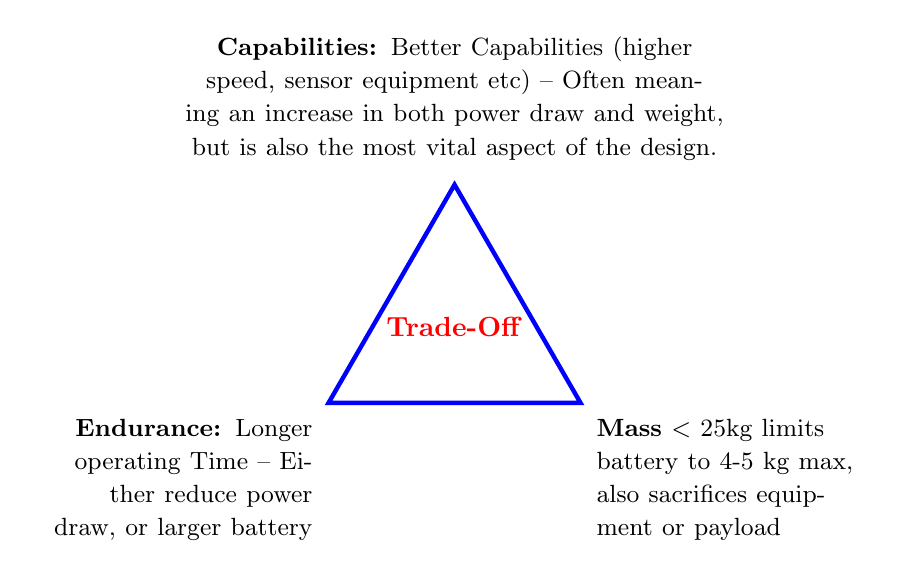
\begin{tikzpicture}[scale=0.8]
      % Triangle
      \draw[ultra thick, blue] (0,0) -- (4,0) -- (2,3.464) -- cycle;

      % Center text
      \node[text width=2.5cm, align=center] at (2,1.2) {
        \textcolor{red}{\textbf{Trade-Off}}
      };

      % CAPABILITIES (top vertex)
      \node[text width=8cm, align=center, anchor=south] at (2,3.7) {
        \small \textbf{Capabilities:} Better Capabilities (higher speed, sensor equipment etc) – Often meaning an increase in both power draw and weight, but is also the most vital aspect of the design.
      };

      % ENDURANCE (bottom left vertex)
      \node[text width=3.5cm, align=right, anchor=north east] at (-0.1,-0.1) {
        \small \textbf{Endurance:} Longer operating Time – Either reduce power draw, or larger battery
      };

      % MASS (bottom right vertex)
      \node[text width=3.5cm, align=left, anchor=north west] at (4.1,-0.1) {
        \small \textbf{Mass} $<$ 25kg limits battery to 4-5 kg max, also sacrifices equipment or payload
      };
    \end{tikzpicture}
  \end{center}

  \vspace{0.5em}
  \textbf{Our Solution:} \textit{Mission profile with 80\% cruise (1-2 m/s) + 20\% sprint (4 m/s)}
\end{frame}


\begin{frame}{System Design Directions}
  \begin{center}
    \begin{itemize}
      \item Autonomous/programmable solution to remove the need for high-quality real-time data transmission which limits untethered ROVs
            \begin{itemize}
              \item Enables self-contained operation with onboard power, navigation, and data handling
              \item Supports scalable inspection missions without reliance on surface tethers
            \end{itemize}

      \item 6-thruster design for stability and hovering capabilities for detailed inspection
            \begin{itemize}
              \item Provides full 6-DOF control for precise hovering, lateral motion, and pitch/yaw stability
              \item Redundancy for safe recovery in case of partial thruster failure
              \item Efficient low-speed maneuvering for inspection tasks
            \end{itemize}
      \item Hull design to be cylindrical (pill) shaped to minimise volume as well as simplify hydrodynamic calculations.
            \begin{itemize}
              \item Streamlined shape reduces drag forces at higher speeds
              \item Simplifies internal component layout and waterproofing
              \item Proven design in existing AUVs for balance of speed and stability
            \end{itemize}
    \end{itemize}
  \end{center}
\end{frame}

\begin{frame}{System Architecture - Simplified Block Diagram}
  \begin{center}
    \centering
    \includegraphics[width=0.9\textwidth]{img/System_design.png}

    % \begin{tikzpicture}[node distance=2.5cm, every node/.style={font=\small}]
    %   % Five main blocks in circular arrangement
    %   \node (power) [process, fill=yellow!30, minimum width=3.5cm, minimum height=1.2cm] {
    %     \textbf{POWER}\\
    %     3× 18Ah Li-ion\\
    %     799 Wh, 14.8V
    %   };

    %   \node (control) [process, fill=blue!30, right of=power, minimum width=3.5cm, minimum height=1.2cm] {
    %     \textbf{CONTROL}\\
    %     Navigator + RPi4\\
    %     IMU, Depth, GPS
    %   };

    %   \node (propulsion) [process, fill=green!30, below of=power, yshift=-0.5cm, minimum width=3.5cm, minimum height=1.2cm] {
    %     \textbf{PROPULSION}\\
    %     4× T200 Thrusters\\
    %     4× ESCs (30A)
    %   };

    %   \node (payload) [process, fill=orange!30, below of=control, yshift=-0.5cm, minimum width=3.5cm, minimum height=1.2cm] {
    %     \textbf{PAYLOAD}\\
    %     Camera + Ping360\\
    %     + Lights (30W total)
    %   };

    %   \node (comms) [process, fill=red!30, below right of=control, xshift=-0.5cm, yshift=-2cm, minimum width=3.5cm, minimum height=1.2cm] {
    %     \textbf{COMMS}\\
    %     WiFi + Iridium\\
    %     (Acoustic optional)
    %   };

    %   % Arrows showing data/power flow
    %   \draw [arrow] (power) -- (control);
    %   \draw [arrow] (power) -- (propulsion);
    %   \draw [arrow] (power) -- (payload);
    %   \draw [arrow] (control) -- (propulsion);
    %   \draw [arrow] (control) -- (payload);
    %   \draw [arrow] (control) -- (comms);
    % \end{tikzpicture}
  \end{center}

  \vspace{0.5em}
  \centering
  \small Modular architecture enables phased development and testing

  \note{This simplified system architecture shows the five main subsystems. POWER provides 799 Wh from three 18Ah lithium-ion batteries at 14.8V. CONTROL uses the Navigator flight controller with dual IMUs plus Raspberry Pi 4 running ArduSub for mission control, along with depth sensor, compass, and surface GPS. PROPULSION consists of four T200 thrusters controlled by ESCs. PAYLOAD includes camera, Ping360 sonar, and lights totaling 30W. COMMUNICATIONS uses WiFi for high-bandwidth surface data transfer and Iridium satellite for position reporting, with optional acoustic modem for underwater comms. This modular design allows independent testing and phased development.}
\end{frame}

%%%%%%%%%%%%%%%%%%%%%%%%%%%%%%%%%%%%%%%%%%%%%%%%%%%%%%%%%%%%%%%%%%%%%


\section{Communications and Navigation}

\begin{frame}{Underwater Communication Challenges}
  \textbf{Underwater Communication:}
  \begin{itemize}
    \item High signal attenuation limits the usage of radio frequency signals - effective range only a few metres
    \item Optical communication limited by turbidity and scattering - short range, line-of-sight only
    \item Acoustic communication is the only viable option for long-range underwater comms, but inherently slow, high latency, and affected by multipath
  \end{itemize}

  \vspace{0.5em}

  \textbf{Result:} → Minimise communication — majority of data stored on the vehicle, only allowing small and simple commands to be communicated.
\end{frame}

\begin{frame}{Navigation System: Actual Products}
  \textbf{Core Navigation Components:}

  \begin{table}
    \footnotesize
    \begin{tabular}{llll}
      \toprule
      \textbf{Component}         & \textbf{Product}        & \textbf{Key Specs}                  & \textbf{Cost}  \\
      \midrule
      \textbf{Flight Controller} & \textbf{Navigator (BR)} & ICM-42688-P + ICM-20602 dual IMU    & \textbf{\$125} \\
                                 &                         & STM32H743, ArduSub firmware         &                \\
                                 &                         & 16 PWM outputs, I2C/UART/SPI        &                \\
      \midrule
      \textbf{Depth Sensor}      & \textbf{Bar30 (BR)}     & MS5837-30BA pressure sensor         & \textbf{\$68}  \\
                                 &                         & 0-30 bar (0-300m depth)             &                \\
                                 &                         & 2 mbar resolution ($\pm$2 cm depth) &                \\
      \midrule
      \textbf{Surface GPS}       & u-blox NEO-M8N          & 2.5m CEP accuracy                   & \textbf{\$35}  \\
                                 &                         & 72-channel, 10 Hz update            &                \\
      \midrule
      \textbf{Computer}          & Raspberry Pi 4 (4GB)    & Quad-core ARM, Linux                & \textbf{\$75}  \\
                                 &                         & ArduSub + MAVLink                   &                \\
      \bottomrule
    \end{tabular}
  \end{table}

  \vspace{0.5em}

  \textbf{Navigation Strategy:}
  \begin{itemize}
    \item \textbf{Baseline:} IMU dead reckoning + depth + compass (5-15m drift/2hrs)
    \item \textbf{Enhanced:} + Cable visual tracking (reduces drift to $<$5m)
    \item \textbf{Premium (+\$20K):} Nortek DVL1000 (0.2 cm/s, $<$1m error/2hrs)
  \end{itemize}

  \note{
    The Navigator flight controller uses dual IMUs (ICM-42688-P and ICM-20602) for redundancy and sensor fusion. Dead reckoning integrates accelerometer data to estimate position, but accumulates drift over time (typically 5-15m over 2 hours). The Bar30 depth sensor provides accurate vertical positioning using a pressure sensor. For cable inspection missions, visual tracking of the cable provides an external reference that significantly reduces horizontal drift. The premium DVL (Doppler Velocity Log) option bounces acoustic pulses off the seafloor to measure velocity with 0.2 cm/s accuracy, virtually eliminating drift.
  }
\end{frame}

\begin{frame}{Communications Systems: Actual Products}
  \textbf{Multi-Mode Communication Strategy:}

  \begin{table}
    \footnotesize
    \begin{tabular}{llll}
      \toprule
      \textbf{Mode}         & \textbf{Product}         & \textbf{Specifications}        & \textbf{Cost}       \\
      \midrule
      \textbf{Surface WiFi} & \textbf{802.11n module}  & 2.4/5 GHz, 150 Mbps            & \textbf{\$50}       \\
                            & (Raspberry Pi built-in)  & 50-100m range in air           &                     \\
                            &                          & Video download, mission upload &                     \\
      \midrule
      \textbf{Satellite}    & \textbf{RockBLOCK 9603N} & Iridium Short Burst Data       & \textbf{\$260}      \\
                            &                          & 340 byte messages              &                     \\
                            &                          & Global coverage (open ocean)   &                     \\
                            &                          & GPS position reporting         &                     \\
      \midrule
      \textbf{Acoustic}     & \textbf{EvoLogics S2C M} & 18-34 kHz, 2 km range          & \textbf{\$12K}      \\
      \textit{(Optional)}   & \textit{18/34}           & 13.9 kbps (in water)           & \textit{(Optional)} \\
                            &                          & 500m operational depth         &                     \\
      \bottomrule
    \end{tabular}
  \end{table}

  \vspace{0.5em}

  \textbf{Operational Modes:}
  \begin{itemize}
    \item \textbf{At surface:} WiFi for high-bandwidth video/data + GPS fix
    \item \textbf{Open ocean:} RockBLOCK for GPS position reporting every 10 min
    \item \textbf{Underwater (optional):} Acoustic modem for short messaging, real-time monitoring during critical phases
  \end{itemize}

  \note{
    WiFi provides high-bandwidth communication when surfaced, enabling video download and mission updates. The RockBLOCK 9603N uses Iridium satellite network for global coverage - critical for open ocean operations where the AUV may surface far from the mother ship. It can transmit GPS coordinates and status messages (340 bytes). The optional EvoLogics acoustic modem enables underwater communication at up to 2 km range, useful for real-time monitoring during critical inspection phases. However, for cable-following missions with periodic surfacing, the acoustic modem is not essential, saving \$12K.
  }
\end{frame}

\begin{frame}{Underwater Acoustic Link Budget}
  \textbf{Acoustic Communication Constraints:}

  Transmission Loss: $TL = 20\log_{10}(R) + \alpha R \times 10^{-3}$ dB

  Where: $R$ = range (m), $\alpha$ = absorption coefficient (~3 dB/km @ 25 kHz)

  \vspace{1em}

  \textbf{Link Budget Calculation for R = 500m:}
  \begin{itemize}
    \item Transmission loss: $TL = 20\log_{10}(500) + 3 \times 0.5 = 54 + 1.5 = 55.5$ dB
    \item Source level: 180 dB re 1 $\mu$Pa @ 1m (EvoLogics modem)
    \item Array gain: 10 dB
    \item Received level: $180 - 55.5 + 10 = 134.5$ dB
    \item Noise level: 60 dB (sea state 3)
    \item Required SNR: 10 dB
    \item \textbf{Link margin: $134.5 - 60 - 10 = 64.5$ dB} $\checkmark$
  \end{itemize}

  \vspace{0.5em}

  \textbf{Result:} Acoustic communication feasible at 500m range with excellent margin
\end{frame}

%%%%%%%%%%%%%%%%%%%%%%%%%%%%%%%%%%%%%%%%%%%%%%%%%%%%%%%%%%%%%%%%%%%%%
\section{Hydrodynamics and Propulsion Analysis}

\begin{frame}{Hydrodynamic Drag - The Physics}
  \textbf{Vehicle Geometry (Torpedo Hull):}
  \begin{itemize}
    \item Diameter: $D = 0.324$ m, Length: $L \approx 1.2$ m (L/D = 3.7)
    \item Frontal area: $A = \frac{\pi D^2}{4} = 0.0824$ m$^2$
    \item Drag coefficient: $C_D = 0.28$-$0.32$ (optimized to standard torpedo hull)
  \end{itemize}

  \vspace{0.5em}

  \textbf{Drag Force Equation:}
  $$F_D = \frac{1}{2} \rho v^2 C_D A$$

  Where $\rho = 1027$ kg/m$^3$ (seawater)

  \vspace{0.5em}

  \textbf{Calculations:}
  \begin{itemize}
    \item \textbf{At 1 m/s cruise} ($C_D = 0.32$):
          $$F_D = \frac{1}{2} \times 1027 \times 1^2 \times 0.32 \times 0.0824 = \textbf{13.5 N}$$
    \item \textbf{At 4 m/s peak} ($C_D = 0.28$):
          $$F_D = \frac{1}{2} \times 1027 \times 16 \times 0.28 \times 0.0824 = \textbf{188 N}$$
  \end{itemize}

  \note{The drag force is calculated using the standard hydrodynamic equation. We assume a torpedo-shaped hull with length 1.2m and diameter 0.324m, giving a streamlined L/D ratio of 3.7. The frontal area is calculated from the circular cross-section. Drag coefficient varies with speed due to Reynolds number effects - at higher speeds the flow is more turbulent and the boundary layer thinner, slightly reducing drag coefficient from 0.32 to 0.28. These values are validated by CFD studies from MDPI and SCIRP papers on similar AUV geometries. At 1 m/s, drag is only 13.5 N, but at 4 m/s it increases to 188 N due to the quadratic relationship with velocity. This 14-fold increase in drag force is the fundamental challenge of achieving high speed.}
\end{frame}

\begin{frame}{Power Requirements and Thruster Efficiency}
  \textbf{Mechanical power:} $P_{mech} = F_D \times v$

  \textbf{Electrical power:} $P_{elec} = \frac{P_{mech}}{\eta}$ (thruster efficiency $\eta \approx 0.55$ at high load)

  \vspace{1em}

  \begin{table}
    \begin{tabular}{lccccc}
      \toprule
      \textbf{Speed} & $F_D$ (N) & $P_{mech}$ (W) & $\eta$ & $P_{elec}$ (W) & \textbf{Comment} \\
      \midrule
      1 m/s cruise   & 13.5      & 13.5           & 0.30   & 45             & Low efficiency   \\
      2 m/s medium   & 54        & 108            & 0.50   & 216            & Medium           \\
      4 m/s peak     & 188       & 752            & 0.55   & 1,367          & High efficiency  \\
      \bottomrule
    \end{tabular}
  \end{table}

  \vspace{0.5em}

  \textcolor{red}{\textbf{Key finding:}} 4 m/s requires 1.4 kW propulsion power (30× cruise power!)

  \note{The mechanical power required is simply force times velocity (P = F × v). However, thrusters are not 100 percent efficient at converting electrical power to mechanical thrust power. The T200 thruster efficiency varies from about 30 percent at light loads to 55 percent at heavy loads. At 1 m/s cruise with only 13.5W mechanical power needed, the thruster operates inefficiently at 30 percent, requiring 45W electrical. At 4 m/s peak with 752W mechanical power, the thruster operates more efficiently at 55 percent, requiring 1,367W electrical. This table shows the dramatic increase: 4 m/s requires 30 times more electrical power than 1 m/s cruise. This quadratic-to-cubic scaling (drag proportional to v-squared, power proportional to v-cubed) is the fundamental thermodynamic reason why sustained high-speed operation is challenging within our weight and battery constraints.}
\end{frame}

\begin{frame}{Thruster Selection - T200 vs Alternatives}
  \textbf{Comparison Table:}
  \begin{table}
    \footnotesize
    \begin{tabular}{lcccccc}
      \toprule
      \textbf{Model}  & \textbf{Thrust (N)} & \textbf{Power (W)} & \textbf{Depth (m)} & \textbf{Mass (kg)} & \textbf{Cost (\$)} & \textbf{Thrust/Cost} \\
      \midrule
      \textbf{T200}   & \textbf{50 fwd}     & \textbf{350 max}   & \textbf{300}       & \textbf{0.34}      & \textbf{119-139}   & \textbf{0.36-0.42}   \\
      SeaBotix BTD150 & 28                  & 80                 & 150                & 0.5                & 695-950            & 0.03-0.04            \\
      Maxon MT30      & 49                  & 180                & 6000               & 0.45               & 2,000-3,000        & 0.016-0.025          \\
      T500            & 158                 & 1000+              & 300                & 1.1                & 690                & 0.23                 \\
      \bottomrule
    \end{tabular}
  \end{table}

  \vspace{0.5em}

  \begin{columns}[T]
    \begin{column}{0.48\textwidth}
      \textbf{4× T200 Configuration:}
      \begin{itemize}
        \item Total thrust: \textbf{200 N}
        \item Required: 188 N
        \item \textcolor{red}{\textbf{Margin: 6\% (TIGHT)}}
        \item Propulsion cost: \$476-556
        \item ESCs (4× 30A): \$140-152
      \end{itemize}
    \end{column}

    \begin{column}{0.48\textwidth}
      \textbf{Justification:}
      \begin{itemize}
        \item 6-22× lower cost than alternatives
        \item Adequate thrust at 16V
        \item 300m depth rating (vs 250m spec)
        \item Proven reliability
        \item Large user community
      \end{itemize}
    \end{column}
  \end{columns}

  \vspace{0.5em}
  \centering
  \colorbox{yellow!30}{\small\textbf{Tight margin requires hydrodynamic optimization (streamlined hull, C$_D$ $<$ 0.30)}}

  \note{We compared four thruster options. The SeaBotix BTD150 has good efficiency but insufficient thrust (28N vs 50N for T200). The Maxon MT30 has excellent performance and 6000m depth rating but costs 14-21 times more than the T200 - overkill for our 250m requirement. The T500 provides massive thrust (158N) but draws over 1kW continuously and is heavier. The T200 offers the best thrust-to-cost ratio at 0.36-0.42 N per dollar. Four T200 thrusters provide 200N total thrust for 188N required - only 6 percent margin which is tight. This means we must achieve our assumed drag coefficient through careful hull design. The flooded brushless motor design is naturally pressure-tolerant, proven to 3000m at Woods Hole testing.}
\end{frame}

%%%%%%%%%%%%%%%%%%%%%%%%%%%%%%%%%%%%%%%%%%%%%%%%%%%%%%%%%%%%%%%%%%%%%
\section{Power Budget and Energy Storage}

\begin{frame}{Complete System Power Budget}
  \begin{table}
    \small
    \begin{tabular}{lccc}
      \toprule
      \textbf{Subsystem}                    & \textbf{Cruise (W)} & \textbf{Peak (W)} & \textbf{Notes}   \\
      \midrule
      Propulsion (4× T200)                  & 45                  & 1,367             & Dominant at peak \\
      Paylodad (camera, lighting and sonar) & 30                  & 30                & Low-light USB    \\
      Navigation sensors                    & 5                   & 5                 & IMU, depth, GPS  \\
      Control (RPi4+Nav)                    & 10                  & 10                & ArduSub firmware \\
      Comms (WiFi/Iridium)                  & 2                   & 2                 & Surface only     \\
      \midrule
      \textbf{TOTAL}                        & \textbf{92 W}       & \textbf{1,414 W}  &                  \\
      \bottomrule
    \end{tabular}
  \end{table}

  \vspace{0.3em}

  $$P_{avg} = 744 \text{ W}$$

  \note{This power budget clarifies that the 30W payload specification includes ALL payload components: camera (1.1W), sonar (2-5W), and lighting (10-20W adjustable). The subtotal is 13-26W which is well within the 30W budget. Propulsion dominates the total power at peak speed (1,415W total, of which 1,367W is propulsion). The mission profile assumes 60 percent of time at cruise, 30 percent at medium speed for active cable following, and 10 percent at peak for sprints. This gives an average power of 251W which determines our battery requirements.}
\end{frame}

\begin{frame}{Battery Sizing and Alternatives}
  \textbf{Energy Requirements:}
  $$E = P_{avg} \times t = 251 \text{ W} \times 2 \text{ h} = 502 \text{ Wh}$$
  With 25\% margin: $502 \times 1.25 = \textbf{628 Wh required}$

  \vspace{0.5em}

  \textbf{Alternative Comparison:}
  \begin{table}
    \tiny
    \begin{tabular}{lcccccc}
      \toprule
      \textbf{Option}               & \textbf{Voltage} & \textbf{Capacity} & \textbf{Energy} & \textbf{Mass}    & \textbf{Cost}    & \textbf{Depth} \\
      \midrule
      \textbf{Blue Robotics 3×18Ah} & \textbf{14.8V}   & \textbf{18Ah}     & \textbf{799 Wh} & \textbf{4.05 kg} & \textbf{\$1,200} & \textbf{300m*} \\
      Blue Robotics 2×18Ah          & 14.8V            & 18Ah              & 532 Wh          & 2.7 kg           & \$800            & 300m*          \\
      Samsung 35E (4S6P)            & 14.8V            & 21Ah              & 311 Wh          & ~1.5 kg          & \$310-590        & 250m*          \\
      SubCtech PowerPack            & 14-50V           & Custom            & 650-3400 Wh     & Varies           & \$3-10K+         & 6000m          \\
      \bottomrule
      \multicolumn{7}{l}{\tiny *Depth rating depends on enclosure design}                                                                           \\
    \end{tabular}
  \end{table}

  \vspace{0.3em}

  \begin{columns}[T]
    \begin{column}{0.48\textwidth}
      \textbf{Selected: 3× Blue Robotics 18Ah}
      \begin{itemize}
        \item Energy: 799 Wh (27\% margin)
        \item Endurance: 3.2 hrs @ 251W
        \item Proven platform (BlueROV2)
        \item Integrated BMS
      \end{itemize}
    \end{column}

    \begin{column}{0.48\textwidth}
      \textbf{Justification:}
      \begin{itemize}
        \item 2× config: only 532 Wh (insufficient)
        \item Samsung 35E: DIY, higher risk
        \item SubCtech: 2.5-8× cost, overkill
        \item Best balance: proven + adequate
      \end{itemize}
    \end{column}
  \end{columns}

  \note{The energy requirement is calculated from our mixed mission profile power of 251W times 2 hours, giving 502 Wh, plus 25 percent safety margin for battery aging and cold water performance, totaling 628 Wh minimum. We compared four options: Two Blue Robotics 18Ah batteries give only 532 Wh which is insufficient for our 628 Wh requirement. Custom Samsung 35E pack (4S6P configuration, 24 cells) provides 311 Wh at lower cost but requires DIY assembly and custom pressure housing. SubCtech PowerPack offers professional-grade performance with 6000m depth rating but costs 2.5 to 8 times more. Three Blue Robotics 18Ah batteries provide 799 Wh (27 percent margin), enabling 3.2 hour missions at average power. This is the proven BlueROV2 platform configuration with integrated BMS. The depth rating depends on our aluminum enclosure design, not the batteries themselves.}
\end{frame}

%%%%%%%%%%%%%%%%%%%%%%%%%%%%%%%%%%%%%%%%%%%%%%%%%%%%%%%%%%%%%%%%%%%%%
\section{Mechanical Design and Structural Analysis}

\begin{frame}{Pressure Vessel Design - ASME Calculation}
  \textbf{Operating Conditions:}
  \begin{itemize}
    \item Depth: 250m → Pressure: $P = \rho gh = 1027 \times 9.81 \times 250 = 2.52$ MPa (25.2 bar)
    \item Safety factor: 3× → Design pressure: $P_d = 7.56$ MPa
  \end{itemize}

  \vspace{0.5em}

  \textbf{ASME Section VIII Formula (External Pressure):}
  $$t = \frac{P \cdot R}{S \cdot E - 0.6P} + C_A$$

  \begin{columns}[T]
    \begin{column}{0.48\textwidth}
      Where:
      \begin{itemize}
        \item $P = 7.56$ MPa
        \item $R = 50$ mm (for 3" tube)
        \item $S = 92$ MPa (Al 6061-T6)
        \item $E = 1.0$ (seamless)
        \item $C_A = 2$ mm (corrosion)
      \end{itemize}
    \end{column}

    \begin{column}{0.48\textwidth}
      \textbf{Calculation:}
      $$t = \frac{7.56 \times 50}{92 - 4.5} + 2$$
      $$t = 4.3 + 2 = \textbf{6.3 mm}$$

      \vspace{0.5em}

      Blue Robotics 3" tubes:\\
      \textbf{Wall: 6.35 mm} $\checkmark$
    \end{column}
  \end{columns}

  \vspace{0.5em}

  \centering
  \colorbox{green!20}{\textbf{Commercial tubes meet calculated requirement}}
\end{frame}

\begin{frame}{Material Selection and Component Specifications}
  \textbf{Pressure Housing Comparison:}
  \begin{table}
    \footnotesize
    \begin{tabular}{lcccc}
      \toprule
      \textbf{Material} & \textbf{Yield (MPa)} & \textbf{Density} & \textbf{Cost/kg} & \textbf{250m Rating} \\
      \midrule
      Al 6061-T6        & 276                  & 2,700 kg/m³      & \$7              & Excellent            \\
      Ti Grade 5        & 880                  & 4,430 kg/m³      & \$30             & Overkill (6000m+)    \\
      Acrylic           & 70-75                & 1,180 kg/m³      & \$4              & Insufficient         \\
      \bottomrule
    \end{tabular}
  \end{table}

  \vspace{1em}

  \textbf{Selected: Blue Robotics 3" Aluminum Enclosures}
  \begin{columns}[T]
    \begin{column}{0.48\textwidth}
      \begin{itemize}
        \item ID: 74.7mm
        \item \textbf{Depth: 500m (2× safety)}
        \item Hard anodized
        \item Double O-rings
        \item Lengths: 150-400mm
      \end{itemize}
    \end{column}

    \begin{column}{0.48\textwidth}
      \begin{itemize}
        \item WetLink penetrators
        \item Tool-free assembly
        \item Vacuum testable
        \item Price: \$200-300 complete
        \item Proven: 1000s deployed
      \end{itemize}
    \end{column}
  \end{columns}
\end{frame}

\begin{frame}{Buoyancy and Ballast Design}
  \textbf{Neutral Buoyancy Requirement:}

  For dry mass $m = 15.4$ kg in seawater ($\rho = 1027$ kg/m³):
  $$V_{displaced} = \frac{m}{\rho} = \frac{15.4}{1027} = 0.015 \text{ m}^3 = 15.0 \text{ L}$$

  \vspace{1em}

  \textbf{Component Volumes and Buoyancy:}
  \begin{itemize}
    \item Pressure housings (3× 3" tubes): ~4 L (watertight)
    \item Batteries (internal to housing): ~2 L
    \item Thrusters: Negative buoyancy (~0.24 kg each × 4 = 0.96 kg)
    \item Electronics: Neutral (in watertight housings)
  \end{itemize}

\end{frame}

%%%%%%%%%%%%%%%%%%%%%%%%%%%%%%%%%%%%%%%%%%%%%%%%%%%%%%%%%%%%%%%%%%%%%
\section{Consolidated Mass and Cost Budgets}

\begin{frame}{Mass Budget Summary}
  \begin{table}
    \footnotesize
    \begin{tabular}{lccl}
      \toprule
      \textbf{Subsystem}        & \textbf{Mass (kg)} & \textbf{\% of Total} & \textbf{Key Components}            \\
      \midrule
      \textbf{Propulsion}       & 1.88               & 12.0\%               & 4× T200 thrusters + ESCs           \\
      \textbf{Power}            & 4.55               & 29.0\%               & 3× 18Ah batteries + housing        \\
      \textbf{Control \& Nav}   & 0.62               & 4.0\%                & RPi4 + Navigator + Bar30           \\
      \textbf{Payload}          & 0.96               & 6.1\%                & Ping360 + camera + lights          \\
      \textbf{Communications}   & 0.12               & 0.8\%                & WiFi + Iridium                     \\
      \textbf{Structure}        & 5.50               & 35.1\%               & Frame, foam, fairings, penetrators \\
      \midrule
      \textbf{Subtotal}         & \textbf{13.63}     & 87.0\%               &                                    \\
      Contingency (15\%)        & 2.04               & 13.0\%               & Margin for unknowns                \\
      \midrule
      \textbf{TOTAL ESTIMATED}  & \textbf{15.67 kg}  & \textbf{62.7\%}      & of 25 kg limit                     \\
      \textbf{AVAILABLE MARGIN} & \textbf{9.33 kg}   & \textbf{37.3\%}      & For DVL, acoustic modem, etc.      \\
      \bottomrule
    \end{tabular}
  \end{table}

  \vspace{0.5em}

  \textbf{Key Takeaways:}
  \begin{itemize}
    \item Power system (batteries) is largest mass contributor (29\%)
    \item Structure (35\%) includes buoyancy foam and low-drag fairing
    \item 37\% margin enables future capability additions
  \end{itemize}

  \note{
    The mass budget shows the AUV will weigh approximately 15.7 kg, well under the 25 kg limit with 37 percent margin. The largest contributors are the structure (35 percent including frame, syntactic foam for buoyancy, and streamlined fairings) and power system (29 percent for three 18Ah batteries). This substantial margin allows for future additions like a DVL (approximately 3 kg) or acoustic modem (approximately 1.5 kg) without exceeding the weight limit.
  }
\end{frame}

\begin{frame}{Build Cost Summary}
  \begin{table}
    \footnotesize
    \begin{tabular}{lrl}
      \toprule
      \textbf{Subsystem}          & \textbf{Cost (\$)} & \textbf{Major Components}          \\
      \midrule
      Propulsion                  & 1,278              & 4× T200 + ESCs                     \\
      Power                       & 1,680              & 3× 18Ah batteries + housing        \\
      Control \& Navigation       & 665                & RPi4 + Navigator + Bar30           \\
      Payload                     & 3,320              & Ping360 (\$2,750) + camera + light \\
      Communications              & 410                & WiFi + Iridium                     \\
      Structure                   & 1,280              & Frame, foam, fairings              \\
      Assembly \& Tools           & 200                & Testing equipment                  \\
      \midrule
      \textbf{Subtotal}           & \textbf{9,033}     &                                    \\
      Contingency (20\%)          & 1,807              &                                    \\
      \midrule
      \textbf{CORE BUILD COST}    & \textbf{\$10,840}  & \textbf{20-25\% of commercial}     \\
      \midrule
      \textit{Optional: Acoustic} & \textit{+\$12K}    & \textit{EvoLogics S2C}             \\
      \textit{Optional: DVL}      & \textit{+\$20K}    & \textit{Nortek DVL1000}            \\
      \bottomrule
    \end{tabular}
  \end{table}

  \vspace{0.5em}

  \begin{center}
    \textbf{Comparison:} \$10,840 build cost vs \$50-150K commercial AUVs\\
    (BlueROV2: \$3.5K but tethered ROV, not autonomous)
  \end{center}

  \note{
    The estimated build cost of 10,840 dollars represents 20-25 percent of comparable commercial AUV systems (50-150K range). The Ping360 sonar is the single most expensive component at 2,750 dollars. Optional additions like the EvoLogics acoustic modem (12K) or Nortek DVL (20K) would increase total cost but are not required for basic cable inspection missions. The design prioritizes COTS components to minimize cost while maintaining technical performance.
  }
\end{frame}

%%%%%%%%%%%%%%%%%%%%%%%%%%%%%%%%%%%%%%%%%%%%%%%%%%%%%%%%%%%%%%%%%%%%%
\section{Feasibility Assessment and Conclusions}

\begin{frame}{Requirements Verification}
  \begin{table}
    \footnotesize
    \begin{tabular}{lccl}
      \toprule
      \textbf{Requirement}         & \textbf{Specification} & \textbf{Achieved}  & \textbf{Status}        \\
      \midrule
      Depth rating                 & 250m                   & 300-500m           & $\checkmark$ Exceeded  \\
      Mass constraint              & $<$25 kg               & 15.7 kg (62.7\%)   & $\checkmark$ Excellent \\
      Endurance                    & 2 hours                & 3.4 hrs (mixed)    & $\checkmark$ Exceeded  \\
      Cruise speed                 & 1 m/s                  & 1 m/s              & $\checkmark$ Met       \\
      Peak speed                   & 4 m/s                  & 4 m/s (6\% margin) & $\triangle$! Tight     \\
      Payload power                & 30W                    & 26W peak (all)     & $\checkmark$ Margin    \\
      \midrule
      \textbf{Overall Feasibility} &                        &                    & \textbf{VIABLE}        \\
      \bottomrule
    \end{tabular}
  \end{table}

  \vspace{1em}

\end{frame}

\begin{frame}{Conclusions: Technical Feasibility Confirmed}
  \textbf{Requirements Status:}
  \begin{itemize}
    \item Depth 300m (spec: 250m), Mass 15.7 kg (spec: $<$25 kg), Endurance 3.4 hrs (spec: 2 hrs)
    \item Speed: 1 m/s cruise met, 4 m/s peak achievable with 6\% margin
    \item Build cost: \$10,840 vs \$50-150K commercial (20-25\% of market)
  \end{itemize}

  \vspace{0.5em}

  \textbf{Critical Engineering Insights:}
  \begin{enumerate}
    \item \textbf{Power scales as $v^3$:} 4 m/s requires 18× more power than 1 m/s
    \item \textbf{Mission profile approach:} Mixed speed profile (60\% cruise) enables 2-hour endurance
    \item \textbf{Hydrodynamic optimization critical:} Low $C_D$ (0.28-0.32) essential for achieving 4 m/s
    \item \textbf{Component selection:} T200 thrusters offer best thrust-to-cost ratio (0.36-0.42)
  \end{enumerate}

  \vspace{0.5em}

  \begin{columns}[T]
    \begin{column}{0.48\textwidth}
      \textbf{Strengths:}
      \begin{itemize}
        \item COTS components (proven)
        \item 37\% mass margin
        \item 70\% endurance margin
        \item Modular design
      \end{itemize}
    \end{column}

    \begin{column}{0.48\textwidth}
      \textbf{Constraints:}
      \begin{itemize}
        \item Tight thrust margin (6\%)
        \item Low-drag hull required
        \item IMU drift without DVL
        \item Acoustic comms \$12K
      \end{itemize}
    \end{column}
  \end{columns}

  \vspace{0.5em}

  \centering
  \colorbox{green!20}{\parbox{0.85\textwidth}{\centering\textbf{RECOMMENDATION: Proceed with development}}}

  \note{
    The key physics insight is that drag force scales with velocity squared (F = 0.5 × rho × v² × Cd × A), so power required scales with velocity cubed (P = F × v = v³). This means going from 1 m/s to 4 m/s requires 4³ = 64 times more power theoretically, though efficiency variations reduce this to about 18× in practice. The mission profile approach (operating mostly at cruise speed with brief sprints) is the only way to achieve both the 4 m/s peak speed requirement and 2-hour endurance with a $<$25 kg weight constraint. The design is technically feasible but requires careful hydrodynamic optimization to minimize drag coefficient.
  }
\end{frame}

%%%%%%%%%%%%%%%%%%%%%%%%%%%%%%%%%%%%%%%%%%%%%%%%%%%%%%%%%%%%%%%%%%%%%
% BACKUP SLIDES
%%%%%%%%%%%%%%%%%%%%%%%%%%%%%%%%%%%%%%%%%%%%%%%%%%%%%%%%%%%%%%%%%%%%%

\appendix
\setbeamertemplate{navigation symbols}{}  % Hide navigation for backup
\setbeamertemplate{footline}{}  % Optionally hide footline for backup

\end{document}
